\section{Pianificazione}
La pianificazione del lavoro all'interno del gruppo \textit{Zeus Code} segue i canoni dettati nella \hyperlink{scadenze}{sottosezione 1.5}, invece la pianificazione di progetto viene suddivisa nelle seguenti fasi:
\begin{enumerate}
	\item \textbf{Analisi};
	\item \textbf{Consolidamento dei requisiti};
	\item \textbf{Progettazione architetturale};
	\item \textbf{Progettazione di dettaglio e codifica};
	\item \textbf{Validazione e collaudo}.
\end{enumerate}
Ogni fase consiste in un insieme di attività aventi una data di inizio e una di fine, il tutto viene riportato nei diagrammi di Gantt\glo. Viene fissata come data di scadenza il giorno di consegna dei materiali prodotti dalle attività. 
\subsection{Analisi}
\textit{Periodo: dal 2019-01-03 al 2019-04-12}\\
L'inizio di questa fase coincide con la formazione dei gruppi del secondo lotto e la fine corrisponde con la data ultima per la consegna dei documenti relativi alla Revisione dei Requisiti.
Questa fase è stata scomposta nelle seguenti sotto attività:
\begin{itemize}
	\item \textbf{Individuazione degli strumenti}: vengono scelti gli strumenti che saranno impiegati per la parte riguardante le comunicazioni tra membri, vengono inoltre definiti i programmi utili alla scrittura di file \LaTeX; 
	\item \textbf{Norme di Progetto}: utilizzando gli strumenti sopra indicati si stende il documento \textit{Norme di progetto v2.0.0} indipendente dal capitolato scelto. Il documento \textit{Norme di Progetto} viene redatto dall'\textit{Amministratore} per conto del \textit{Responsabile di progetto};
	\item \textbf{Studio di fattibilità}: è compito degli \textit{Analisti} effettuare uno studio dei vari capitolati per evidenziarne pregi e difetti e scegliere il capitolato\glosp da sviluppare. Fase bloccante per l'Analisi dei Requisiti;
	\item \textbf{Analisi dei Requisiti}: questa attività è volta alla produzione del documento \textit{Analisi dei requisiti v2.0.0} relativo al progetto scelto. Questo file è in continua fase di miglioramento fino alla data di consegna;
	\item \textbf{Piano di Progetto}: il \textit{Responsabile} analizza le singole attività e le loro date di scadenza in modo da gestire le risorse necessarie al loro completamento, viene redatto il documento \textit{Piano di progetto v2.0.0};
	\item \textbf{Piano di Qualifica}: attività volta alla redazione del file \textit{Piano di qualifica v2.0.0}, il quale individua le metodologie implicate nel garantire la qualità del prodotto; 
	\item \textbf{Glossario}: documento volto a racchiudere tutti termini che possono risultare ambigui o che semplicemente necessitano di una descrizione appropriata onde evitare incomprensioni;
	\item \textbf{Lettera di presentazione}: questa attività consiste nella redazione della Lettera di Presentazione necessaria  per  la  presentazione del gruppo \textit{Zeus Code} come fornitore.
\end{itemize}

\begin{figure}[H]
	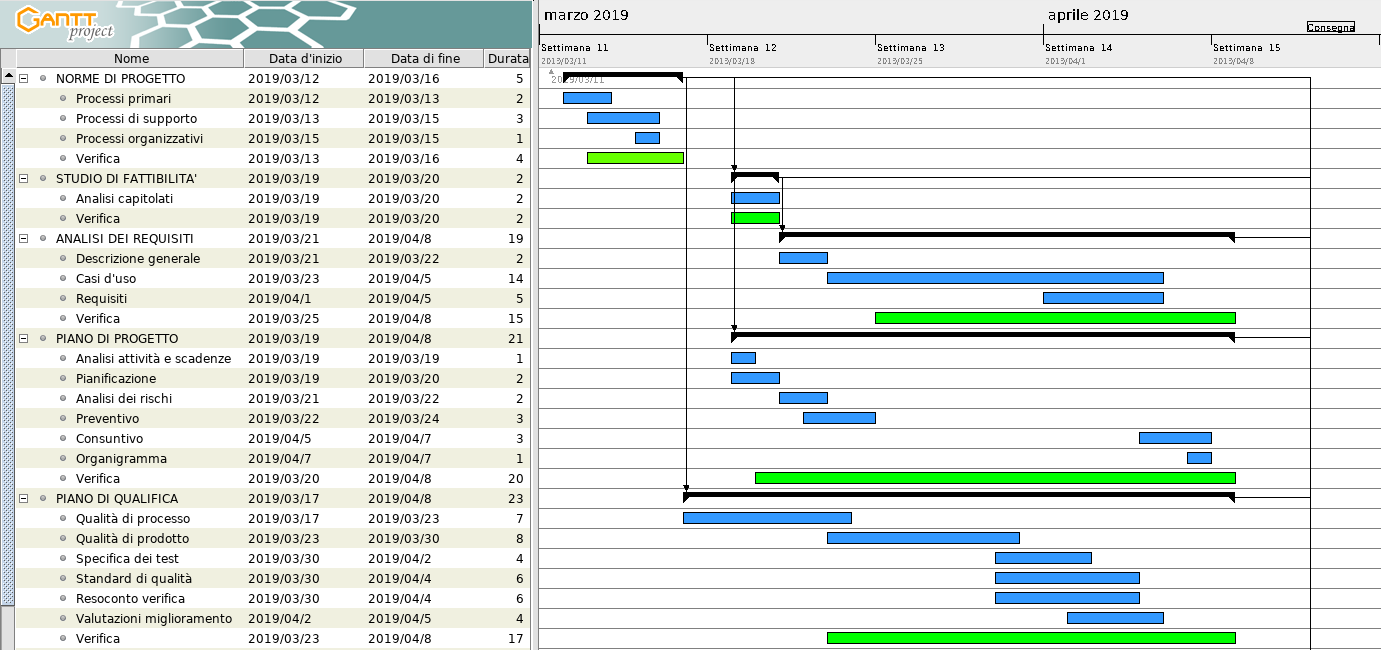
\includegraphics[width=0.99\linewidth]{res/images/gantt_analisi.png}
	
\end{figure}


\subsection{Consolidamento dei requisiti}
\textit{Periodo: dal 2019-04-12 al 2019-04-19} \\
Questa fase ha inizio dopo l'attività di analisi e termina con la presentazione della Revisione dei Requisiti. Le attività 
di questa fase sono:
\begin{itemize}
	\item \textbf{Consolidamento}: vengono migliorati i requisiti ottenuti nella fase di analisi;
	\item \textbf{Preparazione alla presentazione}: viene pianificata la scaletta da seguire per la presentazione del 2019-04-19;
	\item \textbf{Incremento e Verifica}: vengono rivalutati singolarmente tutti i file e in caso saranno soggetti a miglioramenti e modifiche;
	\item \textbf{Approfondimento personale}: i membri del team dedicheranno un monte ore, da loro predisposto, per studiare le nuove tecnologie richieste dal capitolato\glo. Questa attività verrà svolta in modo autonomo e quindi non è riportata nel seguente diagramma di Gantt\glo.
\end{itemize}

\begin{figure}[H]
	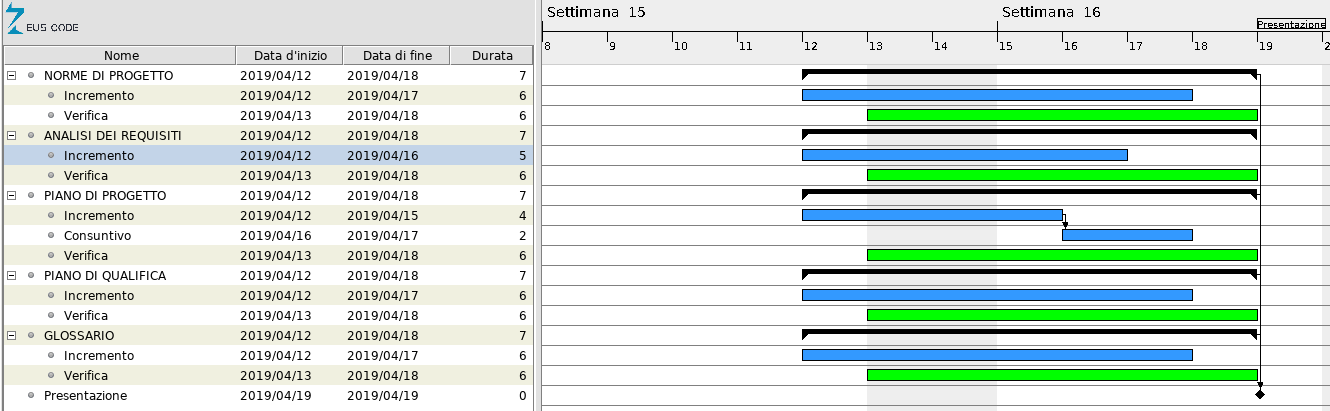
\includegraphics[width=0.99\linewidth]{res/images/gantt_cons.png}
	\caption{Diagramma di Gantt della fase di consolidamento dei requisiti}
\end{figure}

%-----------------Sottosezione Progettazione e codifica per la Technology Baseline---------------------
\subsection{Progettazione e codifica per la technology baseline}
\textit{Periodo: dal 2019-04-20 al 2019-05-10} \\
Il periodo di Progettazione architetturale inizia il giorno successivo alla presentazione per la Revisione dei Requisiti e si conclude con la data di consegna di Revisione di 
Progettazione. In questo periodo le attività principali sono:
\begin{itemize}
	\item \textbf{Incremento e Verifica}: se necessario vengono migliorati i 
	documenti prodotti nelle fasi precedenti;
	\item \textbf{Technology Baseline\glo}: viene codificato il Proof of Concept\glosp il quale viene presentato o condiviso tramite repository\glosp al committente e proponente in una data da definirsi. Tale prodotto è necessario per testare che tutte le tecnologie scelte riescano a soddisfare i requisiti individuati. In questo periodo saranno implementati solo una parte dei requisiti, dando priorità a quelli più importanti e tralasciando la parte riguardante la gamification\glo. Successivamente verranno raffinati i requisiti già definiti, se non completi, e saranno implementate le funzionalità che permetteranno di soddisfare tutti i requisiti.
	Sono stati individuati i seguenti incrementi per facilitare la fase di codifica del Proof of Concept\glo:
	\begin{itemize}
		\item \textbf{Incremento 1 Registrazione:} verrà implementata la registrazione alla piattaforma tramite l'ausilio di Firebase\glo;
		\item \textbf{Incremento 2 Login:} a seguito della registrazione verrà implementata la login;
		\item \textbf{Incremento 3 Inserimento auto:} verrà data la possibilità di inserire una o più auto all'interno dell'applicazione da parte dell'utente;
		\item \textbf{Incremento 4 Visualizzazione auto:} verrà data la possibilità di visualizzare le proprie auto inserite nell'applicazione;
		\item \textbf{Incremento 5 Area personale:} area dell'applicazione dove sarà possibile consultare e modificare i propri dati riguardanti il profilo personale.
		
		
	\end{itemize}
		
\end{itemize}

\begin{figure}[H]
	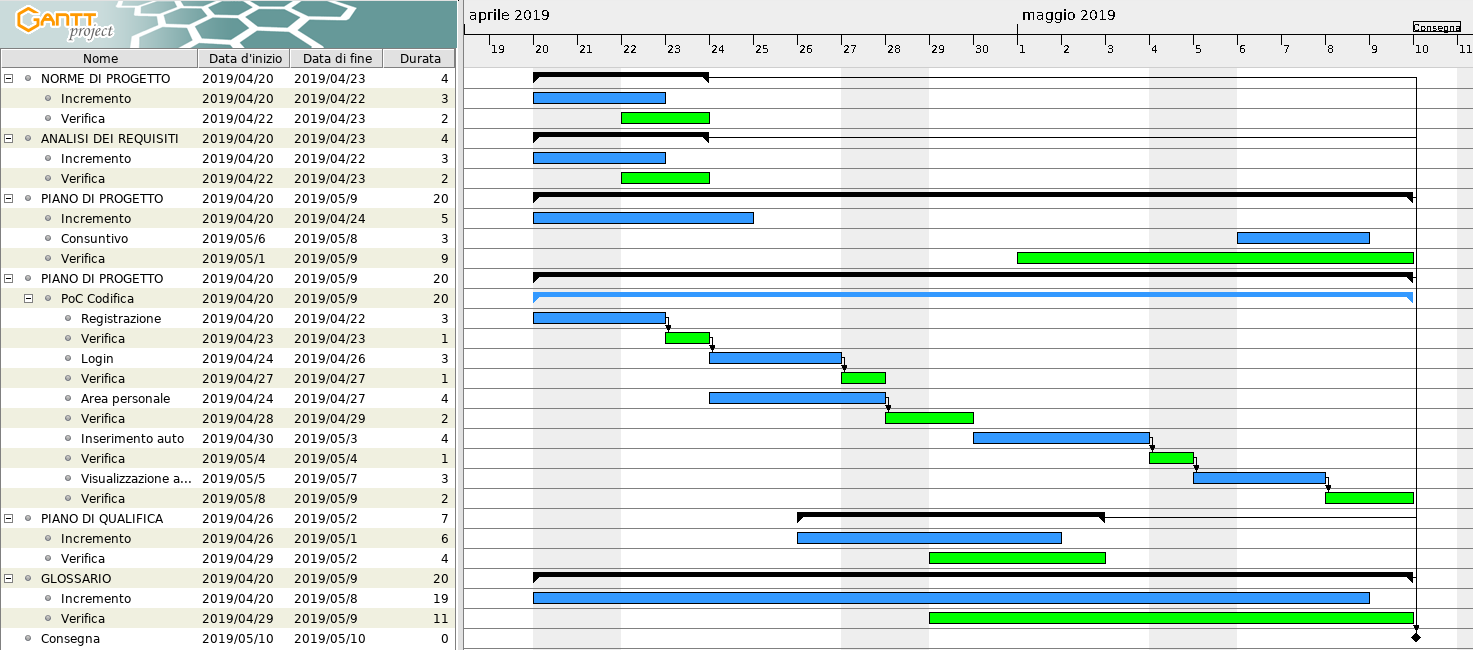
\includegraphics[width=0.99\linewidth]{res/images/gantt_pa.png}
	\caption{Diagramma di Gantt della fase di progettazione e codifica per la technology baseline}
\end{figure}


%-------------------Sottosezione Progettazione di Dettaglio---------------------
\subsection{Progettazione di dettaglio e codifica}
\textit{Periodo: dal 2019-05-18 al 2019-06-10} \\
Il periodo di Progettazione di dettaglio e codifica inizia il giorno dopo la Revisione di progettazione e termina con la data di consegna dei documenti 
in vista della Revisione di Qualifica. Le attività di questa fase sono:
\begin{itemize}
	\item \textbf{Product Baseline\glo}: a seguito della \textit{Technology 
	Baseline\glosp} l'architettura in essa individuata viene scomposta nelle sue unità, ciò permettere di iniziare con la fase di progettazione di basso livello. Segue la redazione del documento Definizione di Prodotto;
	\item \textbf{Codifica}: questa attività consiste nella scrittura del 
	codice e della sua verifica con modalità e strumenti definiti nel 
	\textit{Piano di Qualifica v2.0.0};
	\item \textbf{Manuale Utente}: attività volta alla redazione del documento Manuale Utente, contenente le indicazioni per l'utilizzo del prodotto;
	\item \textbf{Incremento e Verifica}: se necessario vengono migliorati i 
	documenti prodotti nelle fasi precedenti.
\end{itemize}

\begin{figure}[H]
	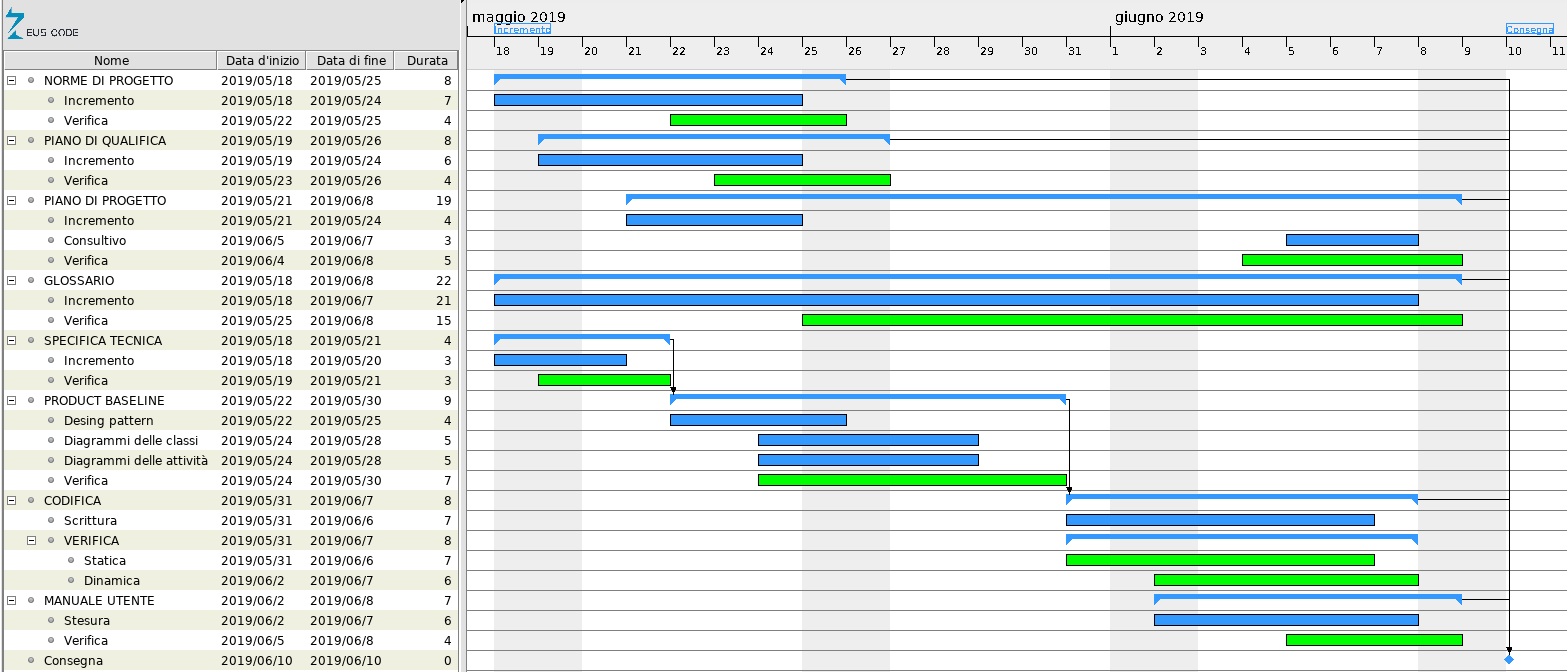
\includegraphics[width=0.99\linewidth]{res/images/gantt_pd.png}
	\caption{Diagramma di Gantt della fase di progettazione di dettaglio e codifica}
\end{figure}
\pagebreak


\subsection{Validazione e collaudo}
\textit{Periodo: dal 2019-06-18 al 2019-07-08 } \\
Il periodo di Validazione e collaudo inizia il giorno successivo alla data di consegna dei documenti per la 
Revisione di Qualifica e si conclude con la data di consegna in vista della Revisione di Accettazione. In questo periodo le attività principali sono:
\begin{itemize}
	\item \textbf{Validazione e Collaudo}: verranno eseguiti test mirati su possibili punti critici del prodotto finito e test generali per valutarne l'effettiva qualità;
	\item \textbf{Manuale Sviluppatore}: viene redatto il documento \textit{Manuale Sviluppatore} atto a fornire tutte le informazioni necessarie al mantenimento, manutenzione e ampliamento del prodotto finale;
	\item \textbf{Incremento e Verifica}: se necessario vengono migliorati i 
	documenti prodotti nelle fasi precedenti.
\end{itemize}
\begin{figure}[H]
	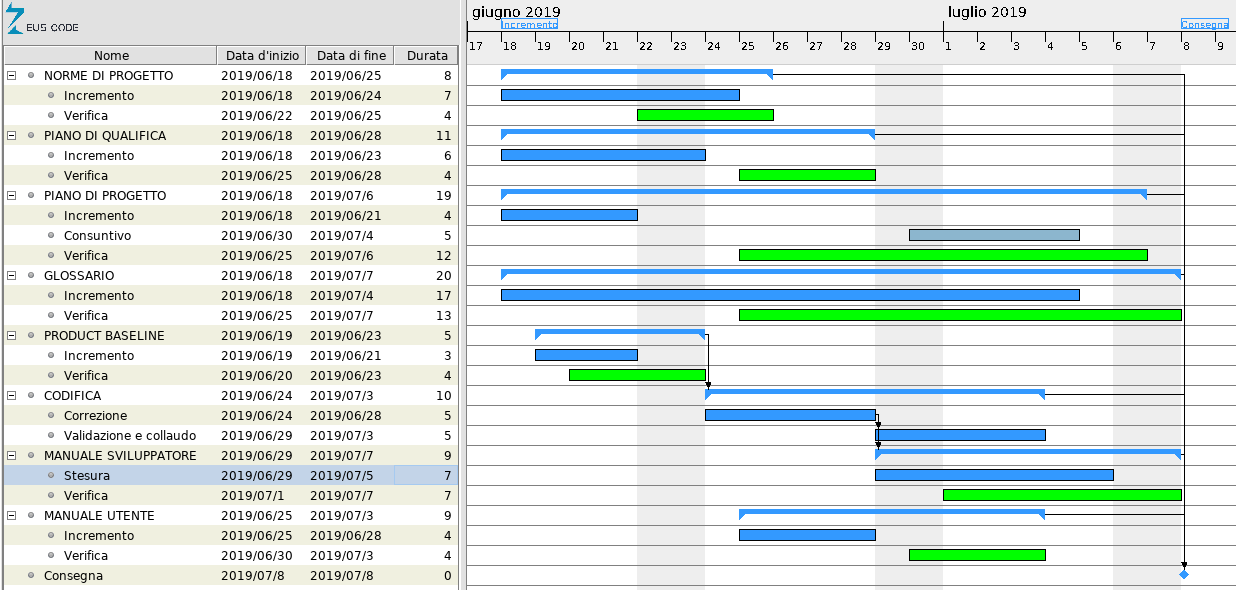
\includegraphics[width=0.99\linewidth]{res/images/gantt_val.png}
	\caption{Diagramma di Gantt della fase di validazione e collaudo}
\end{figure}